%!TEX root = ../sample.tex

\subsection{Correlated POPP}
\label{subsec:cpop}

Recall that Eq.~\ref{eq:independent_sensor_likelihood} is defined under the assumption that each sensor count is conditionally independent from all the others given the true count. This assumption ignores the correlations between sensors. To introduce correlations between sensors we must alter Eq.~\ref{eq:independent_sensor_likelihood} and
Eq.~\ref{eq:joint_binomial_distribution} from the POPP model.

Recall that the probability of a particular sensed count given the true count $P(\mathbf{s_i} \mid c_i)$ was defined from the Poisson limit theorem as a sequence of Bernoulli trials over $l$ subintervals. With correlated sensors, the observation of an event $e_k$ in the $k^{th}$ trial no longer follows the Bernoulli distribution. Instead it follows the categorical distribution, where the $k^{th}$ trial corresponds to whether a particular combination of binary detections $d_{1,k}, \ldots, d_{m,k}$ happens in subinterval $I_k$. Therefore, we move our notation from using $s_{j, i}$ representing sensed counts for particular sensor $j$ independently at time interval $i$ to a matrix representing $m$ sensor detections together at time interval $i$. Formally, we replace Eq.~\ref{eq:independent_sensor_likelihood} and Eq.~\ref{eq:joint_binomial_distribution} with a probability of a series of detection outcomes given the true count $c_i$ at interval $i$ as the following.

We first define for some interval $i$, $l$ subintervals, and $m$ sensors, there is a binary matrix of detections $\mathbf{D^i}$ \footnote{We drop the ($i$) for all notations in this subsection as we will consider a single interval}. $\mathbf{D} \in \mathcal{D}^{m , l}$ the set of binary matrices of dimension $m \times l$. Each column $k$ of $\mathbf{D}$, we denote $\mathbf{D}_{:k} = \mathbf{d} = \{0, 1\}^m$ with $k = 1, \ldots, l$. $\mathbf{D_{:k}}$ is a vector of detections from $m$ different sensors at particular subinterval $k$. 

We further define $e_k \in \{0, 1\}$ as the variable indicating whether or not an event is hypothesized to have occurred in sub-interval $k$. $e_k = 1$ means that an event occurred. We define $P^{+}$ as the categorical distribution of $\mathbf{d}$, conditioned on $e = 1$, i.e.
\begin{equation}
	\label{eq:joint_sensor_model_positive_event}
	P^+(\mathbf{d}) = P(\mathbf{d} \mid e = 1) ~~~~~ \forall \mathbf{d} \in \{0, 1\}^m
\end{equation} 
\noindent and, by analogy,
\begin{equation}
	\label{eq:joint_sensor_model_negative_event}
	P^-(\mathbf{d}) = P(\mathbf{d} \mid e = 0) ~~~~~ \forall \mathbf{d} \in \{0, 1\}^m
\end{equation}
\noindent Both $P^+$ and $P^-$ have $2^m$ elements\footnote{$\mathbf d$ is dropped in the representation unless the context is not clear.}. These two probabilities represent \textit{true positive rates} and \textit{true negative rates}  as $\tau$ and $\xi$ for the POPP model. Similar to $\tau$ and $\xi$, $P^+$ and $P^-$ are estimated from both detections of each sensor and the corresponding actual (non-)event as ground truth. However, unlike $\tau$ and $\xi$ which are sensor specific, $P^+$ and $P^-$ consider all combinations of binary detections from sensors given the true event. This means the number of elements in $P^+$ and $P^-$ grows by a factor of two for each sensor added. Due to the size of $P^+$ and $P^-$, they may need more than a few hundred of detections together with their corresponding events to be estimated.

We can partition the subintervals $1, \ldots, l$ into two sets. $\mathbf{e}^+$ is the set of subintervals $k$ where $e_k = 1$, and $\mathbf{e}^-$ is the set of subintervals $k$ where $e_k = 0$. We can define a partition of the subintervals by a pair $(\mathbf{e}^+, \mathbf{e}^-)$. The set of possible partitions such that $\mathbf{e}^+$ has a fixed size $c$, i.e. $\mid \mathbf{e}^+ \mid = c$, is denoted $\Sigma_c$, so that $(\mathbf{e}^+, \mathbf{e}^-) \in \Sigma_c$.

We further define $\mathbf{D}_{\mathbf{e}^+}$ as an $m \times c$ detection matrix formed from all the columns $\mathbf{D}_{:k}$ where $k \in \mathbf{e}^+$, and $\mathbf{D}_{\mathbf{e}^-}$ as the corresponding $m \times (l - c)$ detection matrix formed from all the columns $\mathbf{D}_{:k}$ where $k \in \mathbf{e}^-$.

As there may be duplicate columns in either or both $\mathbf{D}_{\mathbf{e}^+}$ and $\mathbf{D}_{\mathbf{e}^-}$, we define a count vector for each.
\begin{equation*}
	\mathbf{g}^+ = \textrm{count}(D_{\mathbf{e}^+})
\end{equation*}
\noindent and
\begin{equation*}
	\mathbf{g}^- = \textrm{count}(D_{\mathbf{e}^-})
\end{equation*}
\noindent such that $\sum\limits_{q=1}^{2^m} g_q^+ + \sum\limits_{r=1}^{2^m} g_r^- = l$ where each of $\mathbf{g}^+, \mathbf{g}^-$ are of length $2^m$, having one element for every possible detection vector $\mathbf{d} \in \{0, 1\}^m$.

\begin{figure}[t!]
	\centering
	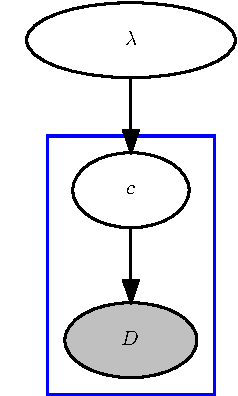
\includegraphics[width=0.2\textwidth]{./figures/cpop-pics.pdf}
	\caption{Graphical representation of C-POPP. Unlike the POPP model, the matrix detection $\mathbf{D}$ represents a joint detection at particular time interval and is affected by the value of the true count $c$, and the sensor rates (joint true positive rate $P^+$ and joint true negative rate $P^-$).} %Furthermore, similar to the POPP-Beta model, the sensor rates are represented by Dirichlet distributions.}
	\label{fig:gm_cpopp}
	\vspace{-20pt}
\end{figure}

In order to define the joint probability of a particular count being yielded by a particular sequence of detection outcomes, we must consider all possible combinations of true positives and false positives that could be generated by that sequence by exploring all elements of $\Sigma_c$. We do this in the following definition of $P(\mathbf{D} | c)$, and define the probability of a given sequence of detection groups yielding count $c$ using the multinomial distribution.
\begin{equation}
\label{eq:codependent_sensor_likelihood}
P(\mathbf{D} \mid c) = \sum\limits_{(\mathbf{e}^+, \mathbf{e}^-) \in \Sigma_c} Mult(\mathbf{g}^+ \mid c, P^+) ~ Mult(\mathbf{g}^- \mid \delta_l c, P^-)
\end{equation}
\noindent with $\delta_l c = (l - c)$.

Eq.~\ref{eq:codependent_sensor_likelihood} can be understood by analogy to Eq.~\ref{eq:joint_binomial_distribution}. In both equations all possible ways pairs of true and false positives counts which sum to $c$ are considered. In the conditionally independent case the binomial distribution is used to determine the probability of each count from the available trials given the true and false positive rates. However, in the conditionally independent case, Eq.~\ref{eq:joint_binomial_distribution} is calculated independently for each sensor, and the joint probability of those sensors results in Eq.~\ref{eq:independent_sensor_likelihood}. In the correlated case the multinomial distribution is used to determine the probability of each count from a possible sequence of joint observations and their probability of yielding a count. With that, Eq.\ref{eq:codependent_sensor_likelihood} removes the need of Eq.~\ref{eq:independent_sensor_likelihood} in C-POPP model. A graphical representation for C-POPP can be seen in Figure \ref{fig:gm_cpopp}.

One should note that the benefit of C-POPP is that it exploits correlations among multiple sensors contributing to detection counts. If there is only one sensor counting events, then C-POPP collapses to POPP.


%\subsection{The Correlated POPP}
%\label{subsec:cpop}
%
%Recall that Eq.~\ref{eq:occurrences_likelihood} is defined under the assumption that each sensor count is conditionally independent from all the others given the true count. This assumption ignores the correlations between sensors. 
%% 
%To introduce correlations between sensors we must alter Eq.~\ref{eq:independent_sensor_likelihood} and
%Eq.~\ref{eq:joint_binomial_distribution} from the POPP model.
%
%
%To replace Eq.~\ref{eq:joint_binomial_distribution}, recall that the probability of a particular sensed count was defined from the Poisson limit theorem as a sequence of Bernoulli trials over $l$ subintervals.
%% 
%With correlated sensors, the observation of an event $e_k$ in the 
%$k^{th}$ trial no longer follows the Bernoulli distribution. Instead it follows the categorical distribution, where the $k^{th}$ trial corresponds to whether a particular combination of binary detections $d_{1,k}, \ldots, d_{m,k}$ happens in subinterval $I_k$. Therefore, instead of having independent sensor models for the detection of event $e_k$ we propose the joint observation model:
%\begin{equation}
%\label{eq:joint_sensor_model}
%P_{jnt}(\mathbf{d_k} ; e_k)
%\end{equation}    
%\noindent where $ \mathbf{d_k} = (d_{1,k}, \ldots, d_{m,k})$, with $d_{j,k}$ being a detection by sensor $j$ in the $k^{th}$ subinterval, and $d_{j,k}, e_k \in {0, 1}$. 
%
%From this we define functions $\mathcal E^+, \mathcal E^- : \mathbf{d} \rightarrow [0,1]$ which provide the probability of a joint observation given that $e_k$ occurred or did not, respectively. 
%
%\begin{equation}
%\mathcal E^+ = P_{jnt}(\mathbf{d_k} ; e_k=1)
%\end{equation}
%\begin{equation}
%\mathcal E^- = P_{jnt}(\mathbf{d_k} ; e_k=0)
%\end{equation}
%
%
%% \textbf{NOTE: Probably not needed but this implies that the value of each function over all $\mathbf{d_k}$ sums to 1. \emph{$\mathcal E^+$ and $\mathcal E^-$, each sums up to 1. These $\mathcal E^+$ and $\mathcal E^-$ are basically the TPR and TNR in these joint observation/sensor models}}
%
%Recall that the set of detections for observation period $i$ was defined as:
%\begin{equation*}
%\mathbf{s_i} = (s_{1i}, \ldots, s_{mi})
%\end{equation*}
%with $s_{j,i} \in \mathbb N$, the sensed count of sensor $j$ from the $i$-th observation period. Since the joint observation model is defined under a combination of binary detections of sensors, each $s_{j,i}$ can be split into $l$ subintervals such that in each sub interval $I_k$ there is only one detection $d_{j,k}$. If the binary detections from all sensors at subinterval $I_k$ are grouped together, then for the observation period $i$, $\mathbf{s_i}$ can be alternatively defined as a list of $l$ \emph{detection groups} of binary detections:
%\begin{equation}
%\label{eq:s_i_definition}
%\mathbf{s'_i} = ((d_{1,1}, \ldots, d_{m,1}), \ldots, (d_{1,l}, \ldots, d_{m,l}))
%\end{equation}
%\noindent with $d_{j,k}$ being a detection by sensor $j$ at subinterval $I_k$ and $d_{j,k} \in \{0, 1\}$. 
%% Note that this is not a set since detection groups can be duplicated across subintervals.
%
%In order to define the joint probability of a particular count being yielded by a particular sequence of detection groups, we must consider all possible combinations of true positives and false positives that could be generated by that sequence. We do this in the following definition of $P(\mathbf{s_i} ; c_i)$, and define the probability of a given sequence of detection groups yielding count $c_i$ using the multinomial distribution.
%
%\begin{equation}
%\label{eq:codependent_sensor_likelihood}
%P(\mathbf{s_i} ; c_i) = \sum\limits_{\mathbf{s} \in \mathcal{P}(\mathbf{s'_i})} Multi(\mathbf{s} ; |\mathbf{s}|, \mathcal E^+) ~ Multi(\mathbf{s'_i}\setminus \mathbf{s} ; (c_i - |\mathbf{s}|), \mathcal E^-)
%\end{equation}
%
%\noindent where $\mathcal{P}(\mathbf{s'_i}) = 2^{\mathbf{s'_i}}$, i.e. the list all possible combinations of size $n$ from of elements of $s'_i$\footnote{We have used the powerset symbol, $\mathcal{P}$, since it provides an indication of the entity being created. However note that we are not working with sets since $\mathbf{s'_i}$ can contain multiple identical sequences of $d_{j,k}$.}. 
%
%% \textbf{NOTE: \emph{Is using powerset correct? How do we distinguish the total number of each $(d_{1,1}, \ldots, d_{m,1}$?}}
%
%Eq.~\ref{eq:codependent_sensor_likelihood} can be understood by analogy to Eq.~\ref{eq:joint_binomial_distribution}. In both equations all possible ways pairs of true and false positives counts which sum to $c_i$ are considered. In the conditionally independent case the binomial distribution is used to determine the probability of each count from the available trials given the true and false positive rates. In the correlated case the multinomial distribution is used to determine the probability of each count from a possible sequence of joint observations and their probability of yielding a count.
%
%One should note that the benefit of C-POPP is that it exploits correlations among multiple sensors contributing to detection counts. If there is only one sensor counting events, then the POPP model is more computationally efficient.
